
% This LaTeX was auto-generated from MATLAB code.
% To make changes, update the MATLAB code and republish this document.

\documentclass{article}
\usepackage{graphicx}
\usepackage{color}
\usepackage{amsmath}
\usepackage{amssymb}
\usepackage[a4paper, total={6in,8in}]{geometry}
\usepackage{pdfpages}

\sloppy
\definecolor{lightgray}{gray}{0.5}
\setlength{\parindent}{0pt}

\begin{document}


\includepdf{../TitlePage.pdf}
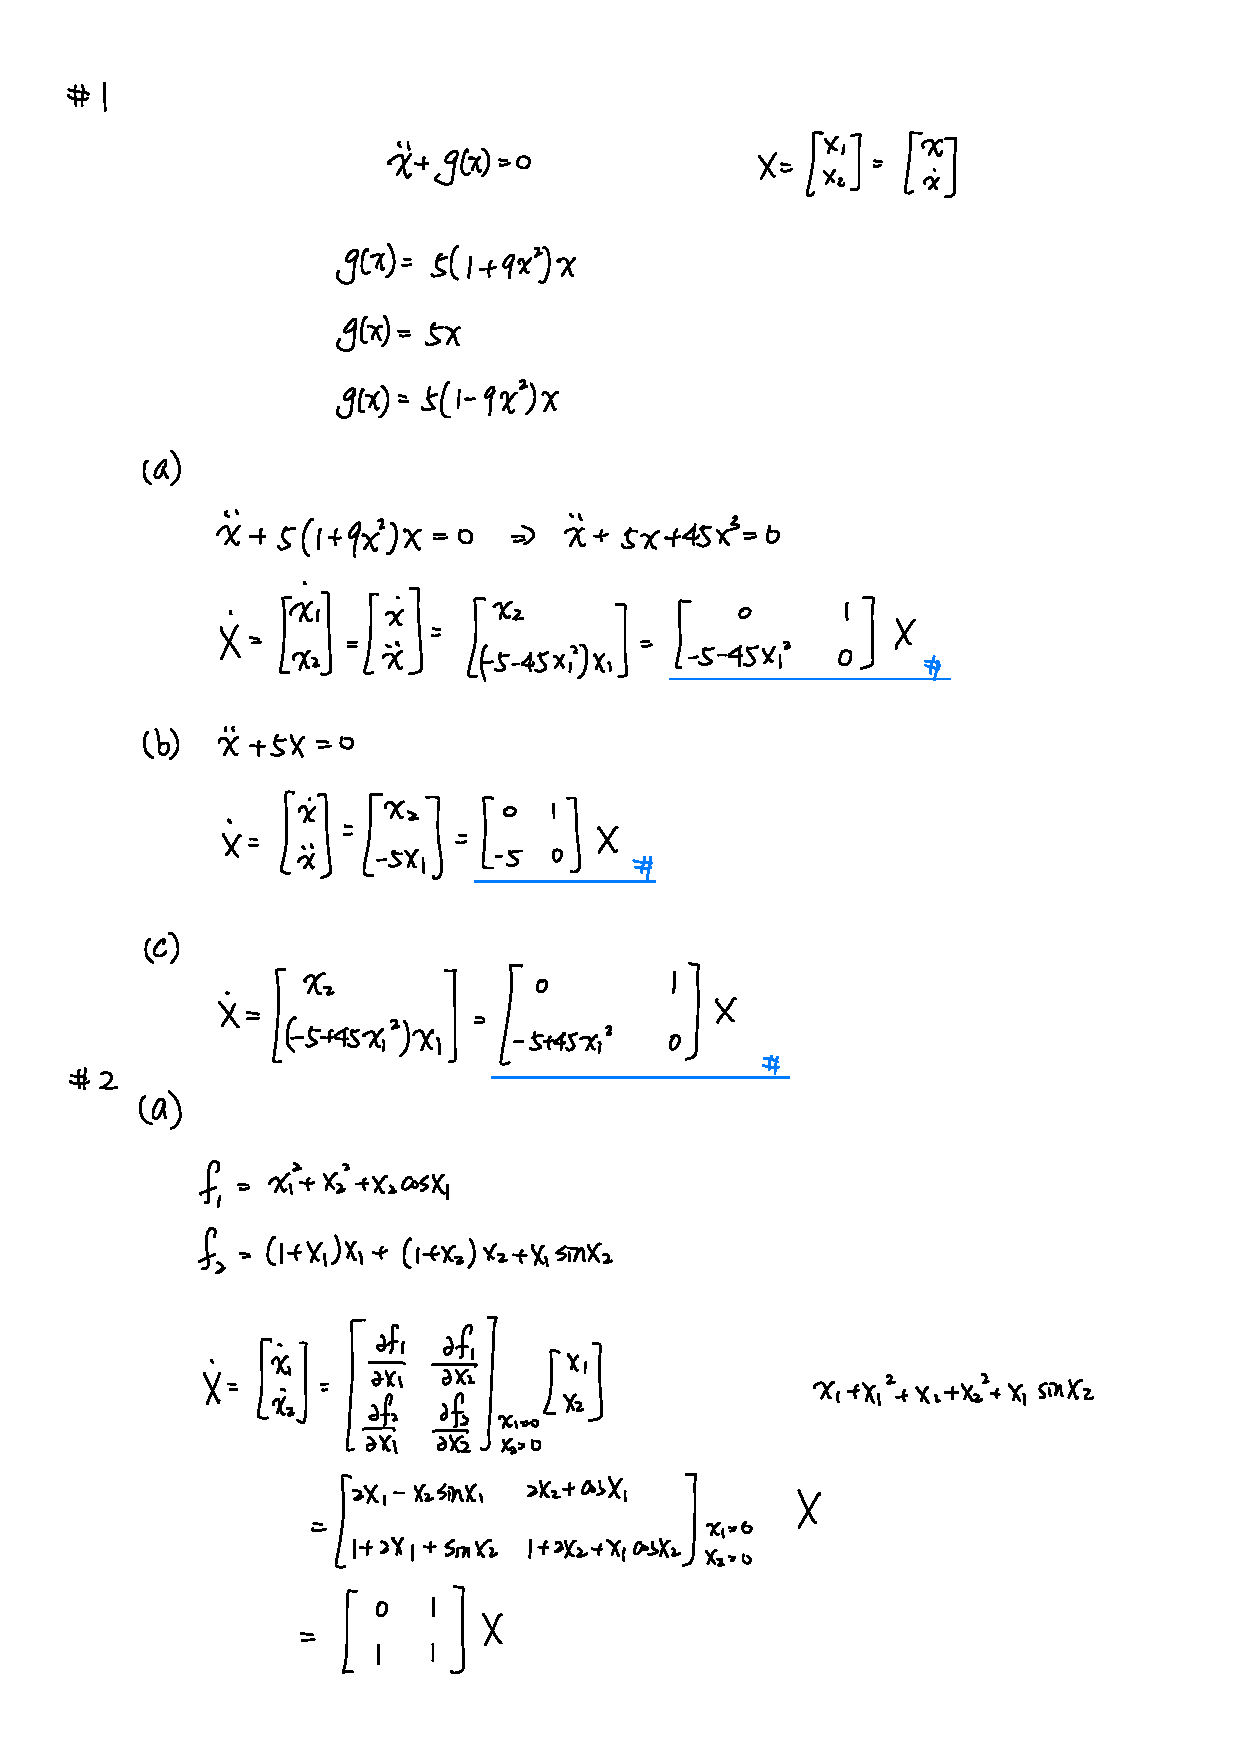
\includepdf[pages=-]{handout.pdf}

\section*{Script}

\subsection*{\#1(a)}

\begin{verbatim}
clear;clc;close all
odefun = @(t, x) [0 1; -5-45*x(1)^2 0]*x;

[~, x] = ode45(odefun, [0 10], [1 0]);

figure()
plot(x(:,1), x(:,2))
grid on
daspect([1 1 1]); axis([-6 6 -6 6])
xlabel("$x$", "Interpreter", "latex"); ylabel("$\dot{x}$", "Interpreter", "latex")
\end{verbatim}

\begin{center}
        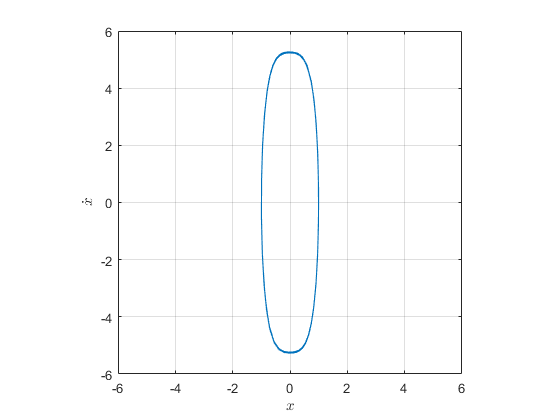
\includegraphics [width=4in]{HW1_01.png}
\end{center}

\subsection*{\#1(b)}

\begin{verbatim}
clear;clc;close all
A = [0 1; -5 0];
odefun = @(t, x) A*x;

[~, x] = ode45(odefun, [0 10], [1 0]);

figure()
plot(x(:,1), x(:,2))
grid on
daspect([1 1 1]); axis([-3 3 -3 3])
xlabel("$x$", "Interpreter", "latex"); ylabel("$\dot{x}$", "Interpreter", "latex")
\end{verbatim}

\begin{center}
        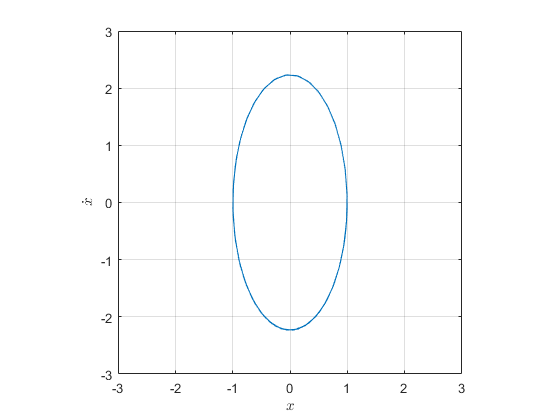
\includegraphics [width=4in]{HW1_02.png}
\end{center}

\subsection*{\#1(c)}

\begin{verbatim}
clear;clc;close all
odefun = @(t, x) [0 1; -5+45*x(1)^2 0]*x;

[~, x] = ode45(odefun, [0 10], [1 0]);

figure()
plot(x(:,1), x(:,2))
grid on
daspect([1 1 1]); axis([-6 6 -6 6])
xlabel("$x$", "Interpreter", "latex"); ylabel("$\dot{x}$", "Interpreter", "latex")
\end{verbatim}

        \color{lightgray} \begin{verbatim}Warning: Failure at t=2.853162e-01.  Unable to meet integration tolerances
without reducing the step size below the smallest value allowed (8.881784e-16)
at time t.
\end{verbatim} \color{black}

\begin{center}
        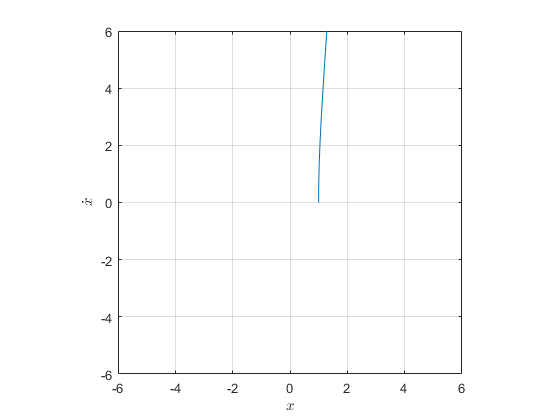
\includegraphics [width=4in]{HW1_03.png}
\end{center}

\subsection*{\#2(a)}

\begin{verbatim}
clear;clc;close all
nonlinear = @(t, x) [x(1)^2+x(2)^2+x(2)*cos(x(1)); (1+x(1))*x(1)+(1+x(2))*x(2)+x(1)*sin(x(2))];
linear = @(t, x) [0 1 ; 1 1]*x;

[t_linear, x_linear] = ode45(linear, [0 1], [0.1 0]);
[t_nonlinear, x_nonlinear] = ode45(nonlinear, [0 1], [0.1 0]);

figure()
plot(t_linear, x_linear(:,1), t_nonlinear, x_nonlinear(:,1))
grid on
legend("linear", "non-linear")
xlabel("$t$", "Interpreter", "latex"); ylabel("$x_1$", "Interpreter", "latex")
\end{verbatim}

\begin{center}
        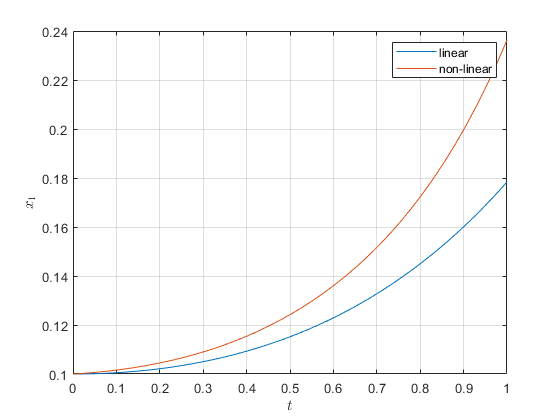
\includegraphics [width=4in]{HW1_04.png}
\end{center}

\subsection*{\#2(b)}

\begin{verbatim}
clear;clc;close all
nonlinear = @(t, x) [x(2); -(3+x(2)^2)*x(2)];
linear = @(t, x) [0 1 ; 0 -3]*x;

[t_linear, x_linear] = ode45(linear, [0 2], [0 0.1]);
[t_nonlinear, x_nonlinear] = ode45(nonlinear, [0 2], [0 0.1]);

figure()
plot(t_linear, x_linear(:,1), t_nonlinear, x_nonlinear(:,1))
grid on
legend("linear", "non-linear")
xlabel("$t$", "Interpreter", "latex"); ylabel("$x_1$", "Interpreter", "latex")
\end{verbatim}

\begin{center}
        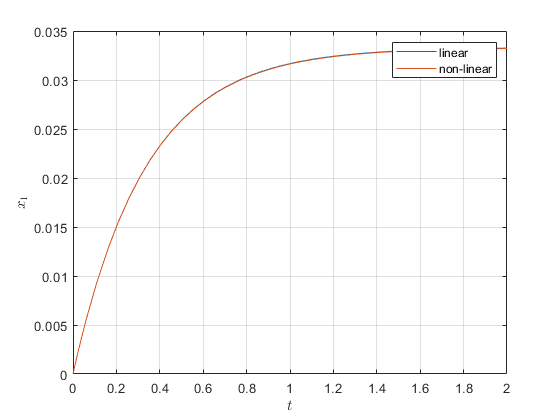
\includegraphics [width=4in]{HW1_05.png}
\end{center}

\end{document}

